\documentclass[conference]{IEEEtran}
\IEEEoverridecommandlockouts
% The preceding line is only needed to identify funding in the first footnote. If that is unneeded, please comment it out.
\usepackage{cite}
\usepackage{amsmath,amssymb,amsfonts}
\usepackage{algorithmic}
\usepackage{graphicx}
\usepackage{textcomp}
\def\BibTeX{{\rm B\kern-.05em{\sc i\kern-.025em b}\kern-.08em
    T\kern-.1667em\lower.7ex\hbox{E}\kern-.125emX}}
\begin{document}

\title{Enhancing Evolutionary Fuzzy Drivers for TORCS using Race-based Selection and BLX--$\alpha$ Crossover}

\author{\IEEEauthorblockN{Mohammed Salem\IEEEauthorrefmark{1},
Antonio M. Mora\IEEEauthorrefmark{2} and
Juan J. Merelo\IEEEauthorrefmark{3}}

\IEEEauthorblockA{\IEEEauthorrefmark{1}Dept. of Computer Sciences, University of Mascara, Algeria. \\Email: salem@univ-mascara.dz}
\IEEEauthorblockA{\IEEEauthorrefmark{2}Dept. of Signal Theory, Telematics and Communications, ETSIIT-CITIC, University of Granada, Spain. \\Email: amorag@ugr.es}
\IEEEauthorblockA{\IEEEauthorrefmark{3}Dept. of Computer Architecture and Computer Technology. University of Granada, Spain. \\Email: jmerelo@geneura.ugr.es}
}

\maketitle

\begin{abstract}

% >>>>>> TODO: Rewrite Abstract -> JJ  <<<<<<<<<<<<<	
	
	



In this paper we will describe a new optimized genetic fuzzy controller for TORCS races So to improve the previous controller presented in CIG conference, we choose to apply $BLX-\alpha$ crossover operator in the genetic algorithm to enhance the optimal solution search process.



\end{abstract}
\begin{IEEEkeywords}
Videogames, Simulated Car Racing, TORCS, Fuzzy Controllers, Autonomous Drivers, Genetic Algorithms, BLX-$\alpha$ Crossover, Optimization, Evaluation
\end{IEEEkeywords}
%%%%%%%%%%%%%%%%%%%%%%%%%%%%%%%   INTRODUCTION   %%%%%%%%%%%%%%%%%%%%%%%%%%%%%%%
%
\section{Introduction}
\label{sec:intro}

% >>>>>> TODO: Rewrite Introduction -> JJ  <<<<<<<<<<<<<
% NEW SELLING POINTS: 
% 	- Tried selection based in races every 5 generations (in addition to at the end)
%	- Implemented BLX-Alpha Crossover to enhance results
%	- Tested against a "real" controller which finished in the middle of classification at the last Car Racing Competition (in 2009, but anyway it has not been improved and it's the only one we have)

Autonomous driving is a problem that shows up in many environments,
including of course self-driving cars, but also in drones, ships,
trains and underwater vehicles. In general, there will be a series of
sensor inputs that include real speed, obstacles and other vehicles,
and based on those sensors, the bot will have to take a decision on
speed and steering that is optimal in several different
senses \cite{Autodriv2006}. Testing different autonomous driving methodologies in real life is usually reserved to just a few big players, and methodologies
as well as algorithms are usually tested in simulated environments;
these simulated environments, at the same time, offer the incentive of
competition among your system and others. In this paper, we will be
using the Open Racing Car Simulator (TORCS) \cite{torcs4}, a very
realistic racing simulator which offers a great testbed for the
implementation and evaluation of autonomous drivers.  
It has been used several times for the celebration of Artificial
Intelligence (AI) competitions, where the aim is to create the best
autonomous driver for racing
\cite{SimulatedCarRacing-2008,oponnents2010,Torcs3,manualTORCS}. Besides being
able to test your car against other cars that have been published, it
can be used as a standalone environment to optimize driving in a
solo race. 

Evolutionary Algorithms (EAs) \cite{EAs_Back96} have been frequently
applied as a general-purpose optimization method in this area,
generally combined with behavioural engines that rule different parts
of the car
\cite{Floreano2004,CarRacing_Pelta09,SAES2012,torcs2012}. These
driving engines have included lately fuzzy controllers
\cite{Guadarrama2008, LFAG, PerezEvolvingFuzzy09}. These controllers
use fuzzy Logic \cite{Fuzzy2011}, a  technique that is quite suitable
for defining this kind of autonomous agents, since they are in part
inspired by the human reasoning when driving. A fuzzy controller works
with linguistic variables, and will for instance turn {\em slightly}
to the right when the next curve is {\em close}, but these controllers
have to be designed to map properly inputs to desired outputs in
particular situations. Previously, the authors presented an approach
combining two specialized fuzzy controllers, designed by hand, that
were able to decide the car's proper steering angle and desired speed
at every single point (or tick) during a race \cite{evo17}. This
driver was later improved \cite{evo18} optimizing the parameters of
their membership functions by means of a Genetic Algorithm
\cite{GAs_Goldberg89}; this automated design improved manual one
obtaining several controllers that were able to beat the initial
hand-designed controller in a race, as well as other published
controllers. 

This proved that evolutionary algorithms were able to get the fuzzy
controller parameters better than a hand-made design, but at the same
time revealed several challenges. In general, evolutionary algorithms
optimize the fitness function that is used; evolved fuzzy controllers
(hereafter FCs) will be eventually as good as the fitness function allows. 
But in this particular case we cannot use as fitness function the position
obtained by the FC in every possible race on every possible track with
every possible opponent, so we have to settle for a {\em surrogate} of
the fitness in a very limited environment. First we opted for
eliminating opponents and making evaluations in solo races; then we
chose a particular track that combined straight segments as well as
some curves and did not take too long to run, and eventually we had to
decide what factors related to speed, damage and lap time were going
to be effectively included in the final fitness function. 

Results were encouraging, but it is still a surrogate model. As such a
model, we need to decide on the best track to perform {\em training}
and also the solo race measures with the biggest impact in the
eventual racing performance. This is why in this paper we have
combined into the fitness function only those terms related with speed during race (to maximize) and damage (to minimize) - the most important factors - in two different approaches.
Besides, the fitness evaluation process has a certain amount of uncertainty because damages and some track conditions can randomly vary in different
evaluations. This is why instead of selecting directly the driver as
we did before, we will be using an actual race among the best drivers
to select the best one.

The main objective of the three new techniques introduced in this
paper, namely, heuristic track selection, fitness function design and
{\em winner} selection have as the main objective to create a better
model of the racing environment. Its results will be commented in the
corresponding section. 

%considering the noisy nature of the problem, which leads to the fact
%that the same individual could obtain very good or very bad results in
%the same races, and against the same opponents, due to the
%stochasticity present in the game and in the rivals' AI.
% Antonio - Just in case we want to comment something about te uncertainty/noise of the game


% Antonio - comment on the results

%Once optimized, the best genetic-fuzzy based controllers (one per fitness) have been evaluated in a practice race (without rivals) first, and then in a real race against different drivers in TORCS. 
%According to the obtained results the enhanced controllers perform both much better than the original fuzzy controller, improving the lap time and reducing the received damage. Moreover they are much more competitive against tough rivals, reaching high ranks in the most difficult races.

The rest of the paper is organized as follows. Next we present the
state of the art, to be followed by a description of the TORCS
simulator, the fuzzy controllers and the Genetic Algorithm implemented in Section \ref{sec:experimental_setup}. After it, the experiments conducted and the obtained results are described in Section \ref{sec:results}. Finally, conclusions and future lines of work will be presented in section \ref{sec:conclusions}.


%%%%%%%%%%%%%%%%%%%%%%%%%%%%%%  STATE OF THE ART  %%%%%%%%%%%%%%%%%%%%%%%%%%%%%%
\section{State of the Art}
\label{sec:soa}

% >>>>>> TODO: Rewrite SotA -> Antonio  <<<<<<<<<<<<<

TORCS has become one of the main environments for research on AI since its launch in 2007 \cite{torcs4}. It offers different kinds of problems to solve, such as the definition of the optimal parameters for the cars (before the race) \cite{Kole-ParamCarTunning12}, and the main one, which is the design of competitive autonomous drivers aiming to win races against other cars, mainly presented in the context on the Simulated Car Racing Competition \cite{SimulatedCarRacing-2008,oponnents2010}.

Evolutionary algorithms have targeted TORCS almost since its
publication, for instance, for determining the
optimal trajectory of a lap in a known circuit \cite{drivingGA2008},
but this approach suffers from the problem that the obtained
trajectory in the evolving process strongly depends on the initial
state of the car.  
In the same context, the authors in \cite{GaRaceLine2010} tried to design a novel approach to compute the optimal racing line without any human intervention, using a GA to find the best trade-off between
the minimization of two conflicting objectives: the length and
the curvature of the racing line.

However, definitely, the most prolific area of application of EAs
inside TORCS has been the optimization of autonomous controllers for
car driving, i.e. conducting a meta-optimization process. 
Thus, EAs have been applied to `refine' the parameters which define
the driver's behavior \cite{ButzCMAES09,SAES2012}, or to improve the
structure/architecture of the models \cite{SAES2012,neurone}, working
offline, or online (during the game)
\cite{TanOnline08,Cardamone_Online_NN}.
% FUZZY + EAs
Our approach is focused in this line, proposing the application of an off-line genetic algorithm for the improvement of the parameters which determine the behavior of a controller for TORCS. We have focused on a Fuzzy-based model, as it is one of the best options for modeling human-like decisions and actions, as others authors have also used this kind of technique in the literature with good results \cite{torcs2012}. 
For instance, in \cite{Guadarrama2008}, a fuzzy rule-based car controller for a Car Racing Competition was built and tuned with co-evolutionary genetic algorithms. Two fuzzy sub-controllers were designed (acceleration and turning angle). But this approach was applied to a simpler simulator than TORCS which is a more realistic and time-constrained simulator. 

P{\'e}rez et al. introduced an evolutionary fuzzy approach for TORCS in \cite{PerezEvolvingFuzzy09}, where they applied EAs for improving fuzzy models to infer the acceleration and turning angle. However, the models were not so specialized as the proposed here, since their controller did not compute the target speed, which is a key factor for a competitive controller. 

Onieva et al. \cite{LFAG} presented a parametrized modular architecture with a fuzzy system and a GA, aiming to reproduce the behavior of a human driver when controlling the steering wheel. In this line, we presented an improved approach \cite{evo17}, which evolved a fuzzy-based driver considering the target speed in addition to the steer (two fuzzy sub-controllers).
This controller was also enhanced in a further work \cite{evo18} optimizing the parameters of the membership functions by means of a real coded genetic algorithm, obtaining a noticeable improvement in performance.

In this paper we focus on the improvement of the evolved controllers by means of a redefinition of the fitness functions, looking for a parameter-less approach (no weights in the terms) \cite{Harik-ParameterLess99}, which will be also more focused on the real objectives for a driver during a race, rather than the overall target. In addition, a `fairer' selection process of the best individual has been implemented, aiming to focus on real good drivers in races, instead of choosing the one with the highest fitness value, which could have a poorer performance due to the uncertainty/noise present on the problem.



%%%%%%%%%%%%%%%%%%%%%%%%%%%%%%  TORCS  %%%%%%%%%%%%%%%%%%%%%%%%%%%%%%

\section{TORCS Simulator and Fuzzy Controllers}
\label{sec:experimental_setup}

The Open Racing Car Simulator (TORCS) \cite{torcs4} is an open
source, modern, multi-player, modular and portable racing simulator
that allows users to compete against other computer-controlled opponents.
Its high degree of modularity and portability, together with the
realistic and real-time driving simulation, make it an ideal testbed
for artificial intelligence research, as we have shown in the previous section.

Every car in TORCS includes  a large set of sensors \cite{Torcs3},
whose values the car can use during a race, such as distances to track borders, to rivals, current fuel, current gear, position in the race, speed, or damage, among others.
The sensor values are considered by any TORCS autonomous driver, or
{\em controller}, to manage the car using actuators \cite{Torcs3}: the
steering wheel, the accelerator, the brake pedal and the gearbox.   

%Thus, a controller is a program, running inside TORCS, that drives a car automatically. It gets as input information about the current state of
%the car and its situation on the track (sensors). These collected data
%are used to decide actions to perform in the next simulation tick.  


\subsection{Fuzzy sub-controllers}
\label{subsec:subcontrollers}

%*****************************  FUZZY CONTROLLER  ******************************
The controller proposed initially \cite{evo17} has the same modular
architecture as the simple TORCS driver; however, the target speed and
steering angle are computed by means of two modular and specialized
fuzzy sub-controllers, which consider five position sensors. This is
the controller which will be improved by means of a GA in this
work.

The {\em fuzzy target speed sub-controller} aims to estimate the
optimal target speed of the car, both in straight parts and curves of
the track, taking into account two criteria: move as fast as possible
and be safe. This estimation is based on two general cases: if the car
is in a straight line, the target speed will take a maximum value
(\textit{maxSpeed} km/h). However, if it is close to a curve, the
controller will decrease the current speed to a value included in the
interval \textit{[minSpeed, maxSpeed]} km/h. 

This fuzzy controller has an output, the speed, and three input values:
\begin{itemize}
	\item Front = Track\_9: front distance to the track border (angle 0\textdegree).  
	\item M5 = max (Track\_8, Track\_10): max distance to the track border in an angle of +5\textdegree and -5\textdegree with respect to Front.
	\item M10 = max (Track\_7, Track\_11): max distance to track border in an angle of +10\textdegree and -10\textdegree.
\end{itemize}

It is a Mamdani-based fuzzy system \cite{iancu2012} with three
trapezoidal Membership Functions (MF) for every input variable. 
%The description of these fuzzy inputs and output are represented in Table
%\ref{tab:flouevar}. 
In \cite{evo18} the different sets of parameters which define the membership functions were improved using a Genetic Algorithm to obtain the best results.

%\begin{table*}
%	\centering
%	{\scriptsize
%		\caption{Fuzzy variables description.}
%		\label{tab:flouevar}
%		\begin{tabular}{ |p{1.5cm}|p{2cm}|p{2cm}|p{2 cm}|p{1 cm}|p{1.5 cm}|p{1.5 cm}|}
%			\hline
%			{ \textbf{Variable}}&
%			{ \textbf{Range}}&
%			{ \textbf{Name}}&  
%			{ \textbf{MF}} &
%			{ \textbf{Low}} &
%			{ \textbf{Medium}}&
%			{ \textbf{High}} \\
%			\hline
%			Input & [0-100] m & Front & trapezoidal & [0-50] & [20-80] & [60-100]
%			\\
%			\hline
%			Input & [0-100] m & M5 & trapezoidal &[0-40] & [10-70] & [50-100] 
%			\\
%			\hline
%			Input & [0-100] m  & M10 & trapezoidal & [0-30] & [20-60] & [50-100]
%			\\
%			\hline 
%			Output & [0-200] m/s & TargetSpeed & singleton & / & / & /
%			\\
%			\hline 
%		\end{tabular} 
%	}
%\end{table*}

% This is from the last paper? If so, just a reference would be
% enough. We need to save space - JJ
% Consider whether adding this again or not -- JJ
% Antonio - not needed

Moreover, the controller is based in a set of fuzzy rules, designed to maximize the car speed depending on the distance to the track border. These rules can be consulted in \cite{evo17}.
% Antonio - TODO: Include the rules if there is available space?
%
%The fuzzy rules are:
%
% \begin{itemize}
% {\small
% 	\item \texttt{IF Front is High THEN TargetSpeed is TS1}
% 	\item \texttt{IF Front is Medium THEN TargetSpeed is TS2}
% 	\item \texttt{IF Front is Low and M5 is High THEN TargetSpeed is TS3}
% 	\item \texttt{IF Front is Low and M5 is Medium THEN TargetSpeed is TS4}
% 	\item \texttt{IF Front is Low and M5 is Low and M10 is High THEN TargetSpeed is TS5}
% 	\item \texttt{IF Front is Low and M5 is Low and M10 is Medium THEN TargetSpeed is TS6}
% 	\item \texttt{IF Front is Low and M5 is Low and M10 is Low THEN TargetSpeed is TS7}\\
% }
%
% In addition, a crisp rule is added to obtain a maximum value of the target speed when the three input variables are as big as possible:\\
% {\small	
% \item \texttt{IF Front = MAXDISTSPEED or M5 = MAXDISTSPEED or M10 = MAXDISTSPEED THEN TargetSpeed = MAXSPEED}
% }
% \end{itemize}
%
% MAXDISTSPEED is the longest possible value for the track sensors, and MAXSPEED is the maximal speed for the specific car. 
% The output value is encoded by seven singletons TS1 to TS7, being respectively: 280, 240, 220, 180, 120, 60 and 30.\\
%
%
% %***********************************************
% \noindent
% \textbf{Fuzzy steering control sub-controller}\\
% %
%
The second is the {\em fuzzy steering sub-controller}, which aims to define the steer angle estimating and determining the target position of the car. 
%
The structure of this sub-controller is similar to the speed one, but it has the steering as output. Thus, the set of sensors considered is the same as in the speed case.

Then, as general rules: if the car is in a straight line, it will set as target position half width of the race track (central position of the lane). Whereas, if the car is near a right curve, it will approach the path leading to the right, with a space between the car and the border of the track to avoid the loss of control. The same approach is considered if the car is near a left curve.

In order to detect the curves, the controller focuses on the sensor values (M10, M5, and Front). So, if the value on Front sensor is the longest, there is a straight road; whereas if the values of M5 and M10 with positive angles (+5 and +10) are the longest, there is right curve; and the other way round.

It uses a base of rules which has been defined trying to model the behavior of a human driver \cite{evo17}.

%, so, for this controller:
% Antonio - TODO: Include the rules if there is available space?

% {\small
% \begin{itemize}		
% 	\item \texttt{IF Front is High THEN steer is S1}
% 	\item \texttt{IF Front is Medium AND M10 is High THEN  steer is S2}
% 	\item \texttt{IF Front is Medium AND M10 is Medium AND M5 is Medium THEN steer is S2}
% 	\item \texttt{IF Front is Medium AND M10 is Medium AND M5 is Low THEN steer is S3}
% 	\item \texttt{IF Front is Low AND M10 is High THEN steer is S3}
% 	\item \texttt{IF Front is Low AND M10 is Medium AND M5 is Medium THEN steer is S4}
% 	\item \texttt{IF Front is Low AND M10 is Medium AND M5 is Low THEN steer is S4}
% \end{itemize}	
% }

% The values for S1 to S4 are respectively: 0, 0.25, 0.5, and 1.
% When M10=Track[7] we will take negative values of the steer (steer=-steer).

% These controllers were defined with our own criteria, but they could be far from being optimal, so, in the following section we apply a Genetic Algorithm for their improvement.


As stated, the designed fuzzy controllers have trapezoidal membership functions given by Equation \ref{eq:trapmf}.
In such a controller, fuzzy rules are applied to linguistic
terms. These terms, which qualify a linguistic variable, are defined
through membership functions, which, in turn, depend on a set of
parameters that `describes' their shape (and operation). Using a GA we
will optimize the parameters of the membership functions that
constitute the fuzzy partition of the linguistic variable
\cite{ThangG08}. The input linguistic variables in our problem,
\textit{Front, Max5} and \textit{Max10}, are represented by three
trapezoidal membership functions. 

A trapezoidal membership function in a finite universe of discourse \textit{[a, b]} can be defined by:

\begin{equation}
\mu_{A}(x)= \left \{
\begin{array}{ll}
\frac{x - x_{1}}{x_{2} - x_{1}},& x_{1} \leq x \leq x_{2}\\
1 , &x_{2} \leq x \leq x_{3}\\
\frac{x_{4} - x}{x_{4} - x_{3}},& x_{3} \leq x \leq x_{4}\\
0        ,& else\\	
\end{array}
\right.
\label{eq:trapmf}
\end{equation}
with:
\begin{equation}
x_{1} \leq x_{2} \leq x_{3} \leq x_{4}
\end{equation}
This MF function is defined by four parameters $x_{1}$, $x_{2}$,
$x_{3}$ and $x_{4}$ taking their values in the interval \textit{[a,
  b]}.% (See Figure \ref{fig:trapeze}).

\begin{figure}[!ht] 
	\begin{center}
		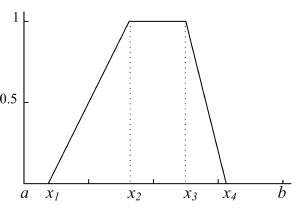
\includegraphics[scale=0.5]{fig/trapese}
		\caption {Trapezoidal MFs}
		\label{fig:trapeze}
	\end{center}
% Mohammed: Could we remove this figure?
% Antonio - if we need space, yes, otherwise, it does not matter I think
\end{figure}
And a fuzzy partition with \textit{n} trapezoidal membership functions
is defined by \textit{2n} variables (\textit{a =} $ x_{1}$,$x_{2}
$,. .., $x_{2n} $ \textit {= b})(Equation \ref{eq:e1}). In this case,
the representation is given by the
figure \ref{fig:at} 
\begin{figure}[!ht] 
	\begin{center}
		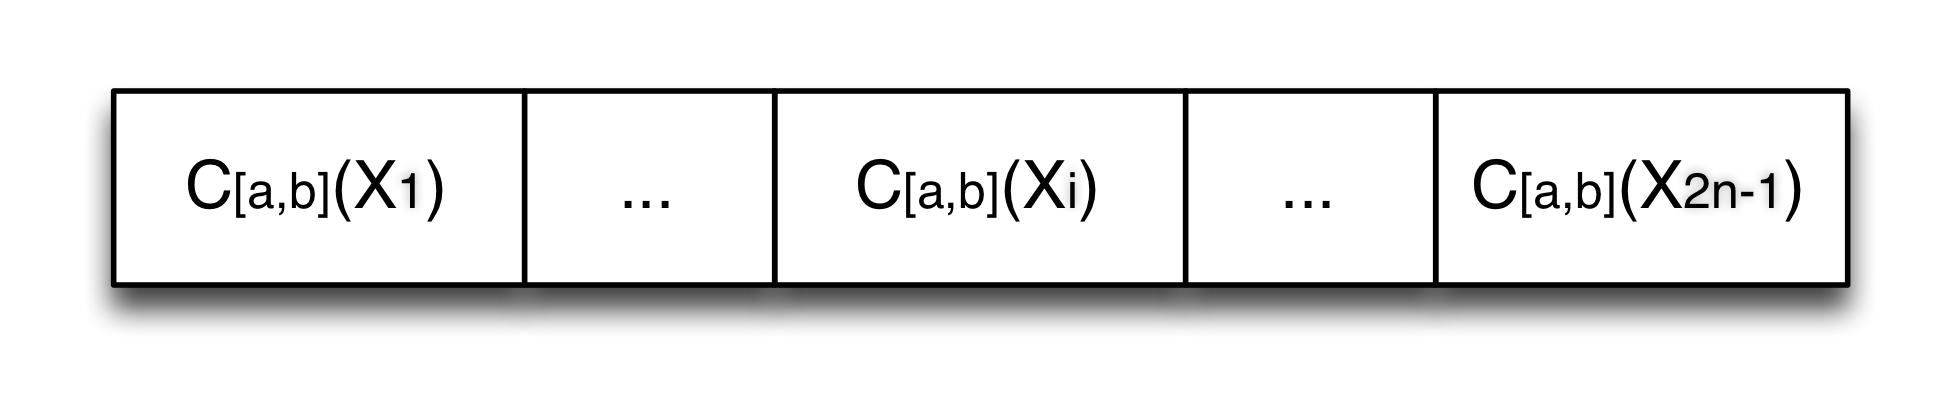
\includegraphics[scale=0.4]{fig/trapezoidal.png}
		\caption {Trapezoidal-shaped MFs coding}
		\label{fig:at}
	\end{center}
\end{figure}
with:
\begin{equation}
a = x_{1} \leq x_{2} \leq...\leq x_{2n-1} \leq x_{2n}=b 	
\end{equation}		

\begin{equation} 
\begin{tabular}{l}
$\mu_{A1}(x)=  \left \{
\begin{array}{ll}
1, &x_{1} \leq x \leq x_{2}\\
\frac{x_{3} - x}{x_{3} - x_{2}}, &x_{2} \leq x \leq x_{3}\\
0        , &x > x_{3}\\
\end{array} 
\right.$		\\ 	
$\mu_{Ai}(x)= \left \{
\begin{array}{ll} 
0, &x \leq x_{2i-2}\\
\frac{x - x_{2i-2}}{x_{2i-1} - x_{2i-2}}, &x_{2i-2} \leq x \leq x_{2i-1},n=2,...,i-1\\
1, & x_{2i-1} \leq x \leq x_{2i}\\
\frac{x_{2i+1} - x}{x_{2i+1} - x_{2i}},& x_{2i} \leq x \leq x_{2i+1}\\
0  , &x > x_{2i+1}\\
\end{array}  
\right.	$		\\
$\mu_{An}(x)= \left \{
\begin{array}{ll} 
0, &x \leq x_{2n-2}\\
\frac{x - x_{2n-2}}{x_{2n-1} - x_{2n-2}},& x_{2n-2} \leq x \leq x_{2n-1}\\
1 ,& x > x_{2n-1} 
\end{array} 
\right.$\\
\label{eq:e1}
\end{tabular}
\end{equation}

This is the base of the optimization conducted by the Genetic Algorithm, as it is described in the following section.


%%%%%%%%%%%%%%%%%%%%%%%%%%%%  OPTIMISING WITH GAS  %%%%%%%%%%%%%%%%%%%%%%%%%%%%

\subsection{Genetic Algorithm}
\label{subsec:GA_optimization}

% >>>>>> Section Rewritten by Antonio - Just missing TODOs by Mohammed  <<<<<<<<

We proposed an optimization approach based in Genetic Algorithms (GAs) \cite{GAs_Goldberg89} aiming to find the optimal parameters of the membership functions of the two sub-controllers previously introduced. 

Thus, every individual is a vector of 18 values/parameters, 6 per variable. Figure \ref {fig:cromosome} illustrates the structure of the chromosome.
\begin{figure*}[!ht]	
  \begin{center}
    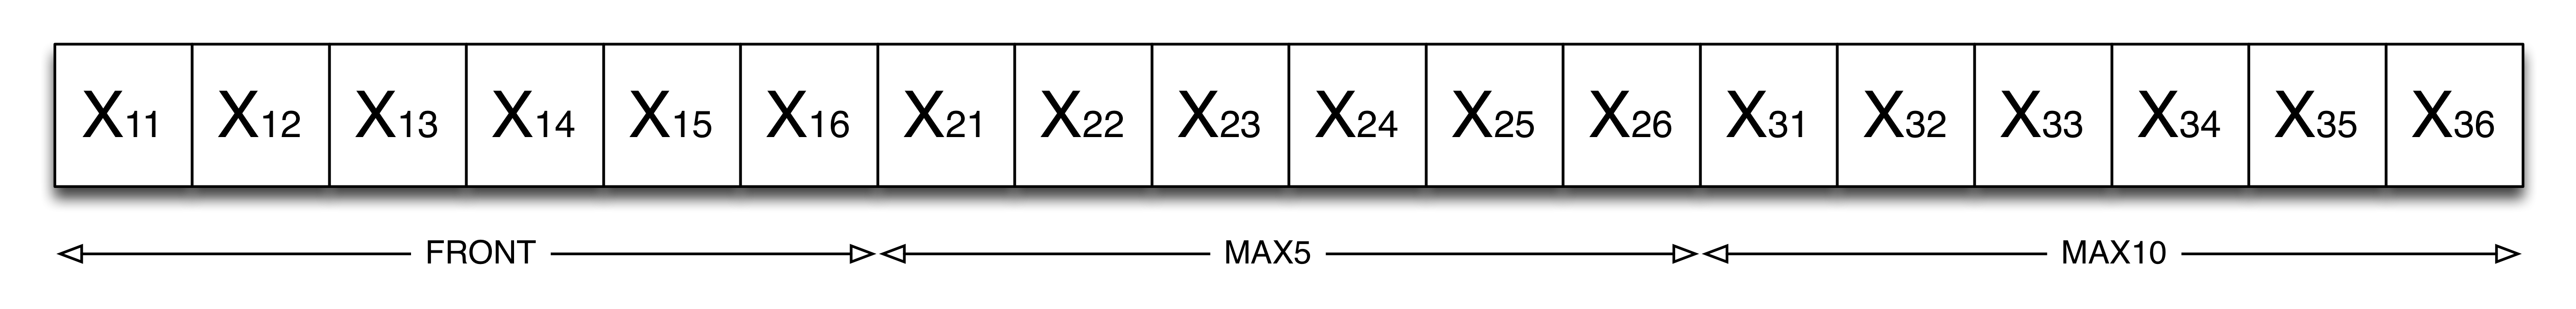
\includegraphics[width=12cm]{fig/chromosome2.png}
    \caption{Chromosome description}
    \label{fig:cromosome}	
  \end{center}	
\end{figure*}

The initialization of the chromosomes (first population) is performed
assigning random values inside a range of variation ($[0,100]$)
\cite{GAs_Goldberg89}, in order to start from feasible values
\cite{evo17}. Since our work requires some precision and the variation interval of each parameter is not well known, we have considered a real coding
implementation \cite{elsayed13} in a vector that includes all variables to optimize.

The overall process is summarized in Figure \ref{fig:ga}. As it can be seen, TORCS is used during the evaluation step of every individual in the evolutionary process.

\begin{figure}[!ht]
  \label{fig:ga}
  \begin{center}
    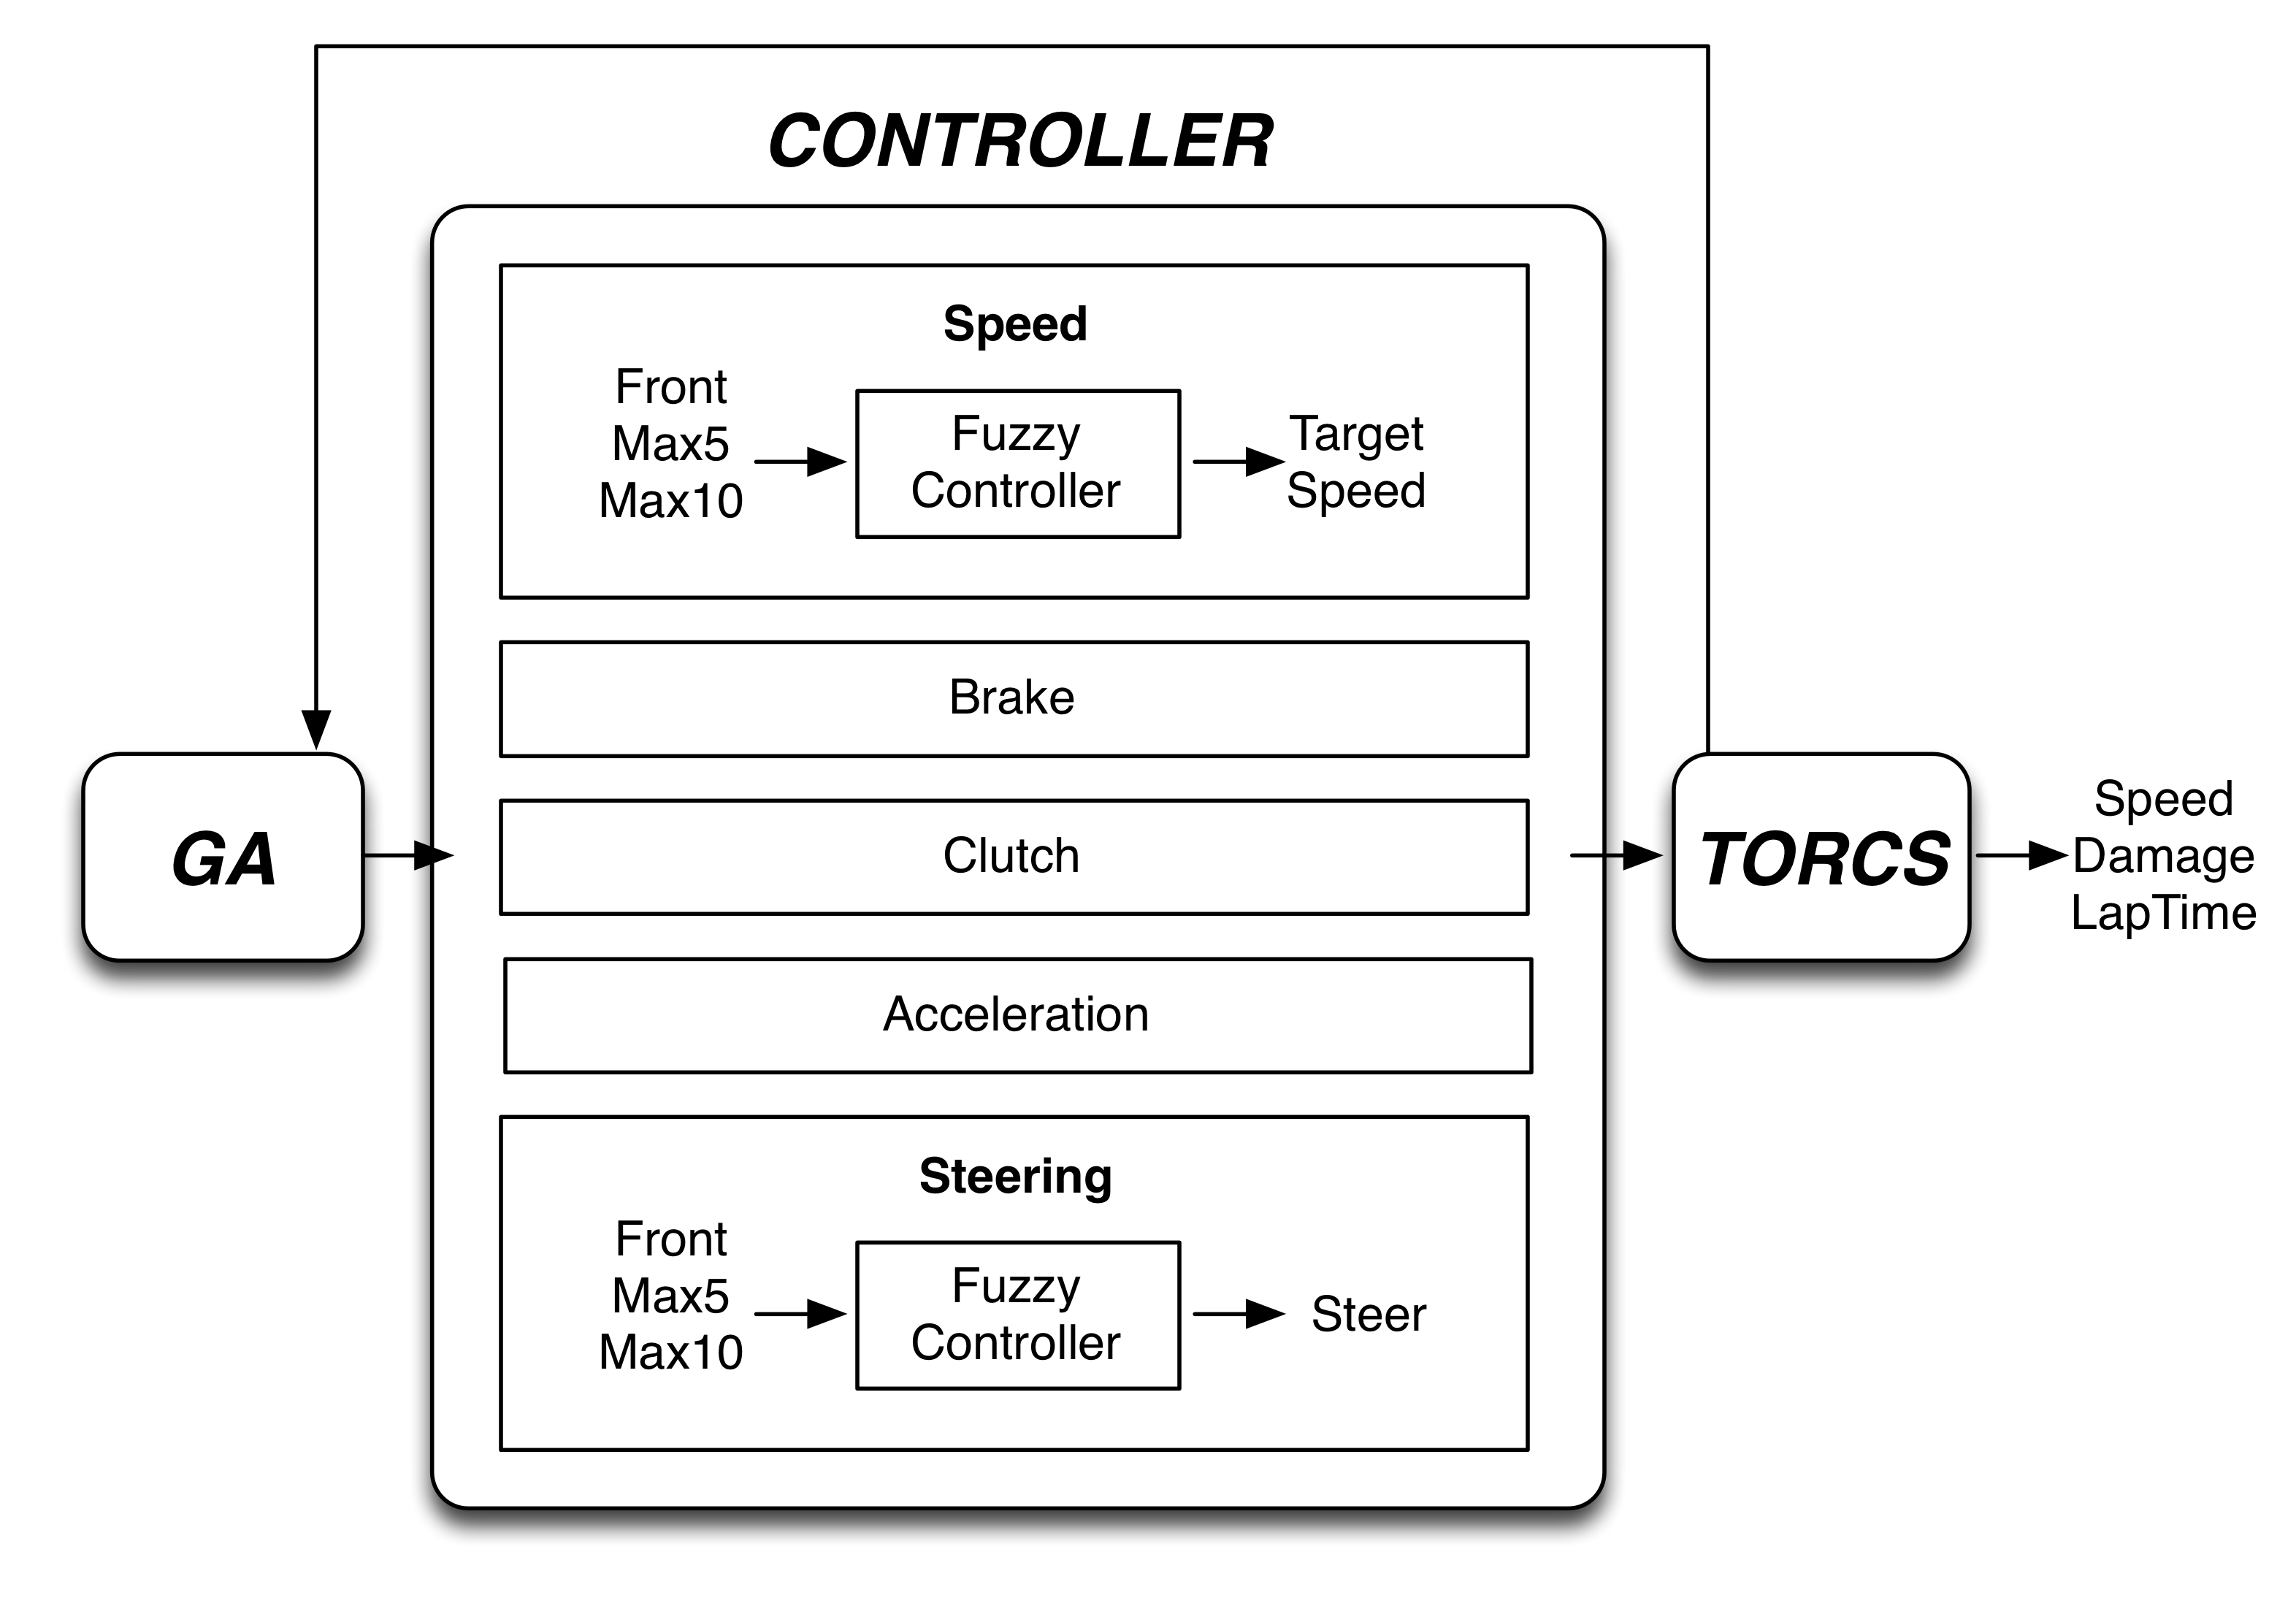
\includegraphics[width=9cm]{fig/flowchart}
  \end{center}
  \caption{Flowchart of  the optimization process of a TORCS fuzzy controller. To evaluate an individual we put the parameter values of the two sub-controllers in the corresponding chromosome, then we launch a race in TORCS with this configuration, obtaining the resulting values of Damage, Top Speed and Mean Lap Time. Individual's fitness value is computed using these values.}
\end{figure}


% TODO: Mohammed, please, revise this

The evaluation of the individuals is based in two different fitness functions (one per approach), namely:
% Antonio - Mohammed, are we still considering two fitness functions?
%%% Mohammed - No only the second one
\begin{description}
	\item[GFC-MMS:]  
	\begin{equation} \label{fit1}
	\begin{array}{ll}
	f_{1} =   \frac{(MinSpeed*MaxSpeed) }{Damage+1}
	\end{array}
	\end{equation}
	\item[GFC-AVS:] 
	\begin{equation} \label{fit2}
	\begin{array}{lll}
	f_{2}= \frac{AVG(Speed)}{Damage+1}
	\end{array}
	\end{equation}	
\end{description}

They depend on some variables, which we considered in our previous work \cite{blind_2018} in order to obtain more `human-like' controllers. So, they try to drive as fast as possible in every single part of the track while avoiding damage. The variables are:
\begin{itemize}
\item $MinSpeed$: aims to increase the good driving in the difficult zones of the tracks (e.g. curves).
\item $MaxSpeed$: centered on the enhancement of the controller in easy or straight parts.
\item $AVG(Speed)$: shows the combination of the overall behavior in the whole track.
\item $Damage$: aims to create `safe' controllers, as it is mandatory being able to finish the race.
\end{itemize} 

So, the fitness of each candidate solution is computed by injecting its gene values to the parameters of the membership functions of the two fuzzy sub-controllers. The defined autonomous controller is used to drive a
car in a 20 laps race in a circuit without opponents, and the results (Maximum, Minimum and Average speed, Damage) are used to compute the fitness value. 
As the objective of the car controller is to win as many races as
possible, we tried to optimize the most general case by carrying out solo {\em training races}, which will be less sensitive to the presence of noise/uncertainty due to the participation of other controllers \cite{unctorcs}.
The selected track for this evaluation will be one with a combination of curves and straight parts in order to obtain an `all-terrain behaviour'.


% >>>>>> TODO: Explain the new selection process -> Mohammed  <<<<<<<<<<<<<

With regard to the other genetic operators, mutation has remained the same as in previous approaches of our genetic controller, i.e. \textbf{non uniform mutation} \cite{mutation1997} has been considered. 

A new \textbf{Race-based Selection process} has been implemented in this approach, aiming to get better individuals/controllers to be parents of the following population. To this end the parents are selected by means of several races against the rest of candidates (X parents compete in each race), the winner of every race is considered as the best of the individuals.
% Antonio - Mohammed, do you conduct just one race among the parents or some of them?
% Mohaammed- we used 5 races to evaluate the X parents
This way, `probably' the best individuals will be selected to reproduce. We cannot assure they are absolutely the best, due to the uncertainty present in this type of environments, i.e. games against non-deterministic opponents\cite{unctorcs}. Anyway, we argue that this selection process will be fairer and more reliable, as it would be desirable in order to ensure a good optimization process.

Due to the high-demanding time this method is, this race-based selection process is just conducted every 5 generations (not in all of them).

% >>>>>> TODO: Explain BLX-Alpha and why we have included it -> Mohammed  <<<<<<

\textbf{BLX-$\alpha$ Crossover operator}\cite{blx2008} has been also added to the GA (instead of previous two-point operator). The blend crossover operator (BLX-α) starts by choosing
randomly a number from the interval $[x_i-\alpha(y_i-x_i).. y_i+\alpha(y_i-x_i)]$, where $x_i$ and $y_i$ are the
$i^{th}$ parameter values of the parent solutions $x$,$y$ and $x_i < y_i$.See Fig\ref{fig:blxalpha}


\begin{figure}[!ht]	
	\begin{center}
		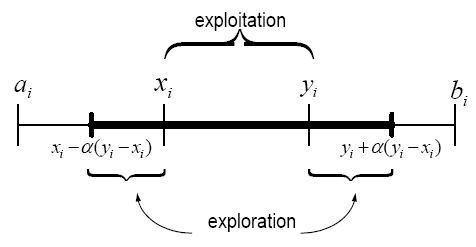
\includegraphics[width=3cm]{fig/blxalpha.jpg}
		\caption{Blend crossover operator ($BLX-\alpha$}
		\label{fig:blxalpha}	
	\end{center}	
\end{figure}



This operator is suitable for real coded genetic algorithms and it achieves a good balance between exploration and exploitation \cite{blx2008}.

This operator is based on the random generation
of genes from the associated neighborhood of the genes in the parents. Thee generated descendants are deferent among them and also among them and their parents leading to a high exploration in the generation of the descendants.

In the Blend crossover operator, the $\alpha$  parameter values can control the exploration/exploitation rate so to
ensure the balance between exploitation and exploration of the
search space, $\alpha = 0.5$ could be selected.

In genetic algorithms, The search process needs high exploration rate in the first generations to explore multiple parts of the search space so to  obtain high diversity but in the last generations, high exploitation is preferred to ensure the optimal solution.
%%Thus, we try to enhance with it.
In our approach, we propose to decrease the values of $\alpha$ so to get more exploitation and less exploitation over the generations. Its value is obtained by \ref{eqalpha}

\begin{equation}
\label{eqalpha}
\alpha =1-\frac{g}{g_{max}}
\end{equation}
where $g$ is the current generation and $g_{max}$ is the maximum generations number.\\
%%Mohammed-  I tried this and it get better results than alpha=0.5
 With this combination, we can achieve an effective
balance between exploitation and exploration and therefore, better solutions may be reached.

This operator is based on the random generation
of genes from the associated neighborhood of the genes in the parents. With
this technique, offspring are generated that can defer
among them and also among them and their parents. In this sense, this operator presents
a high exploration in the generation of the descendants.



%%%%%%%%%%%%%%%%%%%%%%%%%%  NEW RIVAL  %%%%%%%%%%%%%%%%%%%%%%%%%%%%

\section{A New Opponent}  
\label{sec:new-opponent}

% >>>>>> TODO: Describe "S&PL Controller" -> Antonio  <<<<<<<<<<


%%%%%%%%%%%%%%%%%%%%%%%%%%%%  RESULTS  %%%%%%%%%%%%%%%%%%%%%%%%%%%%

\section{Experiments and results}  
\label{sec:results}

% >>>>>> TODO: Explain the new experiments and results -> Mohammed  <<<<<<<<<<
% TODO: Results with Race-based selection (no BLX-Alpha crossover)
% TODO: Results with Race-Based selection and BLX-Alpha crossover
% TODO: Comparison against the standard controllers in TORCS
% TODO: Comparison against S&PL controller (of all our controllers, if possible)




After analyzing most of the available tracks, we have selected for these experiments the \textbf{Alpine 2} circuit. It is a quite complex one, with multiple turns, but also straight parts (See Figure \ref{fig:alpine2_track}).

\begin{figure}[!ht]	
  \begin{center}
    
\includegraphics[width=3cm]{fig/alpine2.jpg}
    \caption{Alpine 2 Track: Slow mountain road. Length: 3773.57m, Width: 10m}
    \label{fig:alpine2_track}	
  \end{center}	
\end{figure}



We have used the driving car  \textit{car1-tbr1} for our controllers, since according to previous experiments \cite{evo17}, this is a fair choice due to its moderate performance. This will lead our controller to be prepared to drive in the most usual conditions. 

We have evaluated the Genetic Fuzzy Controller (GFC) with the proposed fitness functions: $GFC$ (Equation \ref{fit2}). We have run the algorithm with a population size of 60 individuals. The rest of parameters are: Generations=50, Crossover rate=0.85, Mutation rate=0.09, and 10 different runs per configuration.


%\begin{table}[!ht]	
%		\centering
%{\scriptsize
%		\caption{GA parameters}
%		\label{tab:GA_config}
%		\begin{tabular}{|p{3.6cm}|p{3cm}|}
%			\hline \textbf{Population size} & 50 \\
%			\hline \textbf{Generations} & 50   \\
%			\hline \textbf{Crossover rate$\textit{P}_{\textit{c}}$} &  0.85 \\
%			\hline \textbf{Mutation rate $\textit{P}_{\textit{m}}$} &  0.1   \\ 		
%			\hline          
%		\end{tabular}	
%}
%\end{table}

Race  based selection was carried out where 10 races are used to compete every 10 controllers of the population.
We used 5 races (of 5 laps) in the \textbf{Alpine 2} track (used in the optimization) and 5 races (of 5 laps) in \textbf{E-Track 5} track (a new one for them). 
In order to enhance the selection of the best, another two controllers are picked randomly from the default TORCS bots to participate in the race. Moreover, in order to do it fairer, we have defined a \textit{score}, so the controller which gets the fastest lap or the minimum damage in each race is given 5 points.
The evolution process was applied  to obtain the three following controllers:
\begin{itemize}
	\item $GFC$: The controller  from our previous work \cite{blind_2018} using race selection only in the final generation and with fitness of Equation \ref{fit2}.
	\item $GFC-RS$:A controller obtained by applying two points crossover operator and  race selection in every 5 generations and Equation \ref{fit2} in the others. 
	\item $GFC-FA$:A controller obtained by applying $BLX-\alpha$ crossover operator with fixed value of $\alpha$ ($\alpha=0.5$) and race selection in every 5 generations and Equation \ref{fit2} in the others. 
	\item $GFC-VA$:A controller obtained by applying $BLX-\alpha$ crossover operator with a varying value of $\alpha$ using Equation \ref{eqalpha} and race selection in every 5 generations and Equation \ref{fit2} in the others. 
\end{itemize}

These genetic fuzzy based controllers are evaluated in some practice races together with other six bots from TORCS platform.

%"Best laps" and "Min damage" are the scores obtained by every controller in every race when getting the best lap time or/and the minimum damage of all the contenders. 
This evaluation is a kind of Formula 1 mini championship, consisting of 10 races, each one for 20 laps, and with a total of 10 participants per race: the best two $GFC-MMS_1$ and $GFC-AVG_2$, $EVO1$ and $EVO2$, and also 6 bots from TORCS are used to test our controllers. The first 5 races are conducted in \textbf{Alpine 2} track (trained one); and the other 5 races took place in \textbf{E-Track 5} track (not trained for the new controllers, but used in the evolution of our previous ones).
The results are shown in Table \ref{tab:chsresults}. 
%
\begin{table*}[ht]
  \centering
  {\scriptsize
    \caption{ Results of the mini-championship with 10 drivers and 10
      races in two different tracks. {\tt tita}, {\tt berniw} and {\tt
      inferno} are example controllers included with the TORCS
    simulator \cite{torcs4}}
    {
			\begin{tabular}{|c||c|c|c|c|c|c||c|c|c|c|c|c||c|}
				\hline
			&\multicolumn{6}{|c|}{Races in \textbf{Alpine 2} track (20 laps each)} &	\multicolumn{6}{|c|}{Races in \textbf{E-Track 5} track (20 laps each)}&\\
					\cline{2-13}
Driver&{R1}&{R2}&{R3}&{R4}&{R5}&Track Score&{R6}&{R7}&{R8}& {R9}&{R10}&Track Score& Total Score\\
				\hline
$GFC$	&	6&	8&	8&	15&15		&52&	12&	15&	10&	10&	15&62&134\\
$GFC-RS$&	12&	10&	18&	12&12		&64&	10&	8&	12&	25&	8&63&127\\
$GFC-FA$&	18&	12&	15&	10&10		&65&	15&	12&	25&	15&	25&92&157\\
$GFC-VA$&	25&	18&	25&	25&18		&111&	25&	18&	15&	18&18	&94&205\\
$tita1$	&	4&	2&	6&	4&1			&15&	2&	1&	2&	1&	1&7&22\\
$tita2$	&	2&	1&	2&	2&2			&9&	1&	2&	1&	2&	2&8&17\\
$inferno1$&	8&	4&	1&	1&6			&20&	4&	4&	6&	8&	6&28&48\\
$inferno2$&	1&	6&	4&	8&8			&27&	6&	6&	4&	4&	4&24&51\\
$berniw1$&	10&	25&	10&	18&4		&67&	18&	10&	8&	12&	12&60&127\\
$berniw2$&	15&	15&	12&	6&25		&73&	8&	25&	18&	6&	10&67&140\\
\hline
				
			\end{tabular}
		}\label{tab:chsresults}
	}
\end{table*}
%

\textbf{Comparison with S\&PL controller}


Finally, Table \ref{tab:damagespeed} presents a comparison between the  two $BLX-\alpha$ genetic based fuzzy controllers presented in this paper, \textbf{$GFC-FA$} and \textbf{$GFC-VA$} with the S\&PL controller \cite{spl}. The results are the average values of $damage$, $MaxSpeed$ and $Speed$ of 10 races in the \textbf{Alpine 2} and \textbf{E-Track 5} tracks. 

\begin{table}[!ht]
  \centering
  {\scriptsize
    \caption{Average damage and Speed Results of GFC in 5 races in \textbf{Alpine 2} and 5 races in \textbf{E-Track 5} tracks}
    \label{tab:damagespeed}
    \begin{tabular}{|p{1.65cm}|c|c|c|}
      \hline 
      \multicolumn{4}{|c|}{\textbf{Alpine 2}}  \\	
      \hline  
   & \textbf{$GFC-FA$}&\textbf{$GFC-VA$} & \textbf{$SPL$}\\					
      \hline \textbf{Average Speed (km/h)}& 187.11&199.65&176.94\\
      \hline \textbf{Max Speed (km/h)}& 225.07&231.91&217.83\\	
      \hline \textbf{Damage}& 126.82& 117.55&131.99 \\	
      \hline \textbf{Won races}&0&4&1\\	
      
      \hline 
    \end{tabular}
    \begin{tabular}{|p{1.65cm}|c|c|c|}
      \multicolumn{4}{|c|}{\textbf{E-Track 5}}  \\
      \hline 
& \textbf{$GFC-FA$}&\textbf{$GFC-VA$} & \textbf{$SPL$}\\				
      \hline \textbf{Average Speed (km/h)}& 161.11&170.23&160.89\\
      \hline \textbf{Max Speed  (km/h)}&262.88&270.17&266.54\\	
      \hline \textbf{Damage}&18.12& 14.67&28.09\\	 
      \hline \textbf{Won races}&1&3&1\\	
      \hline 
    \end{tabular}
	}
\end{table} 







%%%%%%%%%%%%%%%%%%%%%%%%%%%%  CONCLUSIONS  %%%%%%%%%%%%%%%%%%%%%%%%%%%%
\section{Conclusions and Future Work} 
\label{sec:conclusions}

% >>>>>> TODO: Rewrite this section -> All  <<<<<<<<<<

In this work, we have presented new ways of evaluating controllers
for the TORCS game; these new methods work within an evolutionary
algorithm that optimizes a set of fuzzy controllers for TORCS cars \cite{evo18}. It combines two sub-controllers, one to calculate the target speed and the other for the direction, that is, for driving the steering wheel. 

After initial tests in previous works \cite{evo17,evo18}, that showed the promise of using evolutionary algorithms with two different fitness functions, one considering the average lap time and the car damage and another adding the top speed reached, we discovered the importance of the speed, using different
combinations. {\em A priori}, we could think that races are won by
being very fast when you can be, and trying not to get too slow in
tortuous segments. This heuristic was what drove us to design the
first evaluation function, \textbf{$GFC-MMS$}. However, it could be
thought that sustaining a high average speed will be the most
important factor; this was the heuristic used for \textbf{$GFC-AVS$}. 
The choice of the single track used for training reflected these facts: tracks usually combine ``fast'' and ``slow'' segments, and the car should be able to perform well on both.

Besides, the uncertainty of the evaluation is taken into account when
selecting the {\em best} controller. Since there is a random element
in evaluation, instead of just picking the individual with the best fitness
in the last generation, we select the best ones, make them complete 
against each other and other rivals in a set of real races in several
tracks; then select the one
with the best results overall score. Introducing this element of reality also makes the
choice of controller for comparison a more robust choice than
previously. 

The yielded results are very promising since the optimized controllers
(one per fitness function) were ranked among the first ones in 
different evaluation races with rivals, with the minimum of damage and a very good average and maximum speed. 

In the comparison with the previous evolved fuzzy controllers (from \cite{evo18}), the improvement can be clearly seen in the results. The
new controllers are able to drive much faster than them, even in a
track where the latter were trained, and moreover they manage to
sustain a low damage. They do so even if, compared with
\cite{evo17,evo18}, they are not using damage as a criterium for
optimization. High damage might make a car abandon a race, but
apparently a certain amount of damage should be expected if you want
to win the race. 

At this point, it would be difficult to say which of the three factors
introduced in this paper, namely, new evaluation functions, race track
for evaluation and post-optimization selection of winner, is the one
that contributes the most to the good results. Clearly all three of
them have an impact, but, taking into account the big difference among
results in the post-optimization selection of controllers in the last
generation, probably this step, which deals with uncertainty in the
evaluation of the controller, might have had the biggest
impact. This way of dealing with uncertainty, which is usually a
problem in game bot optimization \cite{merelo2016statistical}, might
be extended in different ways, for instance as a selection method
for all generations.

This is one of the future lines of work, combined with a study of the
influence of all factors in bot performance. This will have to include
tracks, fitness functions and post-optimization selection. This will
have to be combined with the improvement of the controllers
considering a `deeper' and `wider' evaluation (more laps and more
tracks). There is also a similar research line to address, which is the
optimization of the outputs in the fuzzy system, which has been set
manually in all our approaches. 

With regard to the applied GA, it could be improved in different ways,
for instance, reducing its computation time by means of the
parallelization of the evaluation phase. Also, a multi-objective
approach could be implemented, in which the main objectives to address
by the controller could be optimized at once. 
Moreover, we could also try to generate, optimize and tune
automatically the rule base of the fuzzy controller by means of a
Genetic Programming algorithm.  

\section*{Acknowledgments}

This work has been supported in part by: Ministerio espa\~{n}ol de
Econom\'{\i}a y Competitividad under project TIN2014-56494-C4-3-P
(UGR-EPHEMECH), TIN2017-85727-C4-2-P (UGR-DeepBio) and TEC2015-68752 (also funded by FEDER).

\bibliographystyle{IEEEtranS}
\bibliography{fuzzy_torcs}

\end{document}
